\section{Gaze trajectories}
\label{sec:gaze_traj}
%To ground the physical background of this thesis, the present section reviews the physical system we aim to model: the eye-tracking signal which characterises human visual attention. During active vision, the visual system does not operate as a passive receiver of sensory input, but rather as an active, dynamic sampler of a changing environment \cite{friston_does_2018, friston_sophisticated_2021}. This active sensing manifests across two coupled physical observables: the internal dynamics of rich neural oscillatory networks, and the external, mechanical execution of gaze trajectories. Crucially, these domains inform and drive each other, and each exhibit complex, scale-free dynamics in their activity. Characterised by background spectra with power law tails and anomalous diffusion, the visual system is capable of devoting attention to many spatiotemporal scales of event. Viewing these biological phenomena through the lens of statistical mechanics provides a rigorous foundation for mathematically modelling the visual system. This section establishes these empirical constraints by first examining the functional role of neural frequency bands and theta-gamma coupling (\cref{subsec:neur_freq_bands}), before detailing the multi-scale, stochastic regimes of human gaze trajectories (\cref{subsec:gaze_traj}). Together, these behavioural patterns motivate the fractional dynamics given by the FNS equations of motion, and the developments upon that model in the subsequent sections.
Healthy human gaze trajectories are well characterised by a small set of dynamical patterns, the challenge is in understanding their interaction, functional roles, and mechanistic origin. The clearest pattern of gaze trajectories is a division into long jumps in positional attention called saccades, between which are periods of relative stillness called fixations during which information is gathered \cite{erkelens_coordination_2006, seung_how_1996, lencastre_dynamical_2025, benitezy_eyetracking_1970}. Eye-tracking devices---such as the Eyelink 1000 used in collecting data for this thesis as shown in \cref{fig:eye-tracking}\textbf{d)}---provide the high-precision measurements to analyse and model the gaze trajectories through continuous time, both during saccade and fixation.

%This paradigm has a limited history in the literature, and fitting data to a simple jump process called a Lévy flight (see \cref{subsec:levy_motion}) parameterised by the stable parameter $\alpha$ has found some limited use as a biomarker for ADHD \cite{papanikolaou_levy_2024}. Broader saccade metrics based on such jump processes have been found to be valuable as non-invasive biomarkers for broader neural disorders, including schizophrenia \cite{caldani_saccadic_2017, morita_eye_2017, zhu_diagnosis_2024, lindner_disorders_2005, zhu_diagnosis_2024}, autism \cite{bittencourt_saccadic_2013, wang_saccadic_2025}, ADHD \cite{papanikolaou_levy_2024}, and Parkinson's disease \cite{wang_saccadic_2025, bittencourt_saccadic_2013, kaski_ocular_2017}. 

\begin{figure}[b!]
	\centering
	\begin{subfigure}[T]{0.2\textwidth}
		\centering
		\includesvg[width=\linewidth]{figures/schematics/head-schematic-1}
	\end{subfigure}
	\hfill
	% \begin{subfigure}[T]{0.18\textwidth}
	% 	\centering
	% 	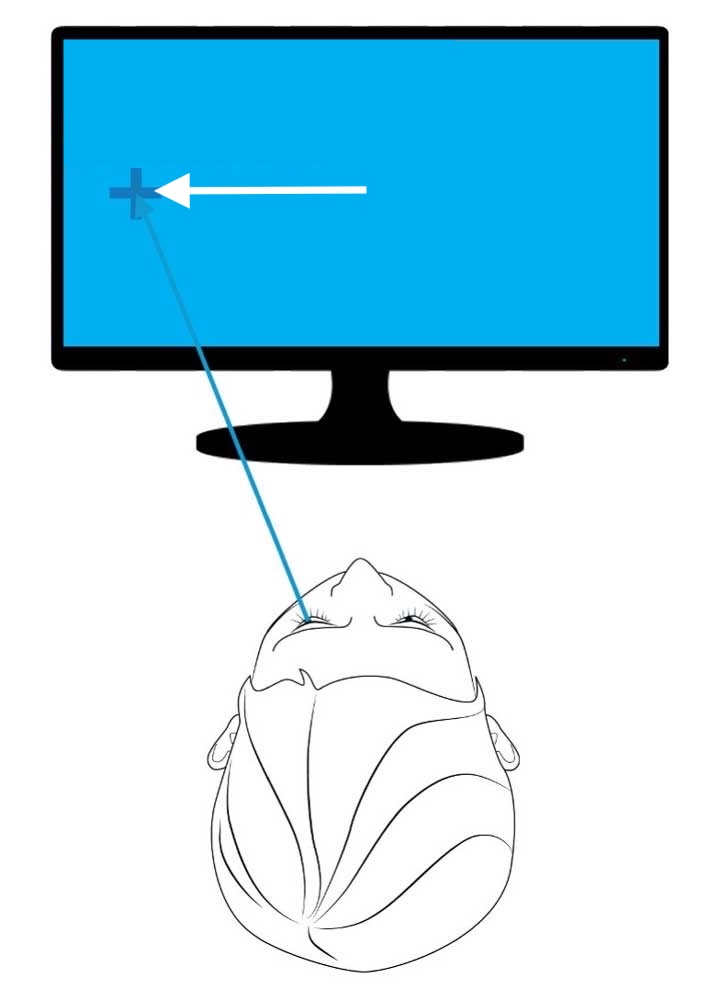
\includegraphics[width=\linewidth]{figures/schematics/head-2.jpg}
	% 	\label{subfig:gamma_fits}
	% \end{subfigure}
	\begin{subfigure}[T]{0.2\textwidth}
		\centering
		\includesvg[width=\linewidth]{figures/schematics/head-schematic-2}
	\end{subfigure}
    \hfill
	\begin{subfigure}[T]{0.2\textwidth}
		\centering
		\includesvg[width=\linewidth]{figures/schematics/head-schematic-3}
	\end{subfigure}
    \hfill
    \begin{subfigure}[T]{0.3\textwidth}
		\centering
		\includesvg[width=\linewidth]{figures/schematics/head-schematic-4}
	\end{subfigure}
	\caption{\textbf{A schematic representation of a typical eye-tracking setup.} \textbf{a)} shows a subject at the beginning of a typical eye-tracking study, with gaze position starting at the centre of the screen $(960, 540)$~\unit{\px}. \textbf{b)} shows a saccade from the centre towards the left of the screen as a target is tracked. \textbf{c)} shows the return of gaze position to the centre of the screen, as the target returns to the centre. \textbf{d)} shows a typical eye-tracking unit, the EyeLink 1000 Plus, as used in the experiment studied in this thesis.\textit{\textbf{a)}--\textbf{c)} are adapted from \cite{srresearch2020eyelink3}, while \textbf{d)} is adapted from \cite{srresearch2013eyelink1000plus}}}
	\label{fig:eye-tracking}
\end{figure}

Where the dynamics of fixation or gaze have been considered, they are treated as separate subject matter to each other, and rarely treated together in single studies. Gaze fixations exhibit three distinct dynamical patterns: near-instant microsaccades within the same point of focus, slow ocular drift about a point of focus, and high frequency ocular micro tremor \cite{van_ede_looking_2026,graham_ocular_2023, engbert_integrated_2011, spauschus_origin_1999}. There are a number of studies examining a rich physical model of fixational dynamics \cite{engbert_integrated_2011, engbert_normal, vasudevan_stochastic_nodate}, as well as developing the role such dynamics have in gathering information efficiently \cite{rucci_control_2015, rucci_miniature_2007, rucci_temporal_2018, rucci_unsteady_2015, roberts_fixational_2013, wu_fixational_2024}.

\subsection{Existing models of visual searching dynamics}\label{subsec:existing_models}
Progress towards modelling gaze dynamics during visual search spans physics, neuroscience, and machine learning. As such, existing models have been built with very different aims and methods. Cognitive and biologically inspired models explain where attention is drawn through biologically-inspired saliency maps and top-down guidance \cite{itti_model_1998, wolfe_guided_2021, Gayet2025-fv}. More normative models ask what an optimally informative searcher would do, selecting saccades by Bayesian belief updating and entropy reduction \cite{najemnik_optimal_2005}. We here examine in detail two influential models representing these two model-making paradigms, those being the self-avoiding random walk model of fixational dynamics presented in \cite{engbert_integrated_2011, Herrmann2017-hw}, and DeepGaze~III from \cite{kummerer_deepgaze_2022} which utilises a deep learning model to predict saccade positions. A full comparison of a selection of influential and successful models, along with a comparison of their core domains, aims, and key features, is given in \cref{tab:search_models_colored} in \cref{app:prior_models}.

The self-avoiding random walk presented in \cite{engbert_integrated_2011} considers the dynamics within a single quadratic potential which confines the gaze into a localised fixation. The gaze position is discretised on a square lattice, and visited positions will increase potential to introduce a self-avoidance condition, which relaxes on a short timescale. Of particular interest to this thesis is the interpretation of the explored potential as a motor map from the neurons in the superior colliculus to motivate a physics-inspired model of gaze \cite{doi:10.1126/science.1166112, CARPENTER2000R291, Sparks2002-zb}. The self-avoidance condition, although taking a different motivation, is mechanistically very similar to the kernel adaptation which we introduce in this thesis to explain rhythmicity in global saccade timings. This work successfully reproduces superdiffusion in fixations, alongside the existence of microsaccades. This model, however, only accounts for fixational motion, and does not aim to capture the long saccades which organise them. Further, although the authors mention tremor, a tremor-frequency peak is not observed in this model.

DeepGaze~III \cite{kummerer_deepgaze_2022} produces fixation prediction through a state-of-the-art deep convolutional neural network, a map of observed oculomotor biases (such as an observed centre-bias in viewing an image), and a history of previous fixations, to predict the location of saccades with the highest accuracy to-date across all metrics considered in the standard MIT/Tübingen Saliency Benchmark \cite{mit-tuebingen-saliency-benchmark, kummerer_deepgaze_2022}. This model is highly successful in fixation prediction, and has been used to research patterns in attention through simulation of saccade prediction without requiring human measurement, however it lacks biological or functional usefulness beyond fixation position. The model provides no temporal information, only providing the location of fixations, and does not consider the dynamics of fixations themselves, nor providing any mapping from biologically realistic neural activity onto the dynamics of gaze.

\subsection{Timescales of neural computation}\label{subsec:neur_freq_bands}
Throughout much of this thesis, links are drawn between model dynamics and well-studied frequency bands of activity in the human brain. It is then valuable to outline the studied computational and functional interpretations of such frequency bands. Neural firing activity is divided into frequency bands named by greek letters, originally discovered and decomposed from electroencephalogram (EEG) data \cite{fan_relation_2007, klimesch_frequency_2018}. Divisions are only approximate, but bands may be thus considered: delta (\SIrange{0.1}{3}{\hertz}), theta (\SIrange{4}{8}{\hertz}), alpha (\SIrange{8}{14}{\hertz}), beta (\SIrange{14}{40}{\hertz}), and gamma (\SIrange{40}{100}{\hertz}) \cite{fan_relation_2007, klimesch_frequency_2018}. Of particular interest to this thesis are the interpretations of theta and gamma neural activity as functionally important to neural computation. Broadly, theta rhythms have been found to modulate and organise bursts in computational gamma-scale neural activity  \cite{qi_fractional_2022, fries_mechanism_2005, fries_rhythmic_2023, fries_rhythms_2015, spyropoulos_theta_2018, bastos_communication_2015}. Theta rhythms have been shown to modulate attention during auditory tasks \cite{wang_attention_2022, yang_neural_2024}, visual search tasks \cite{kawashima_attentional_2022, spyropoulos_theta_2018, Mo_competing_2019}, and when analysing the broad attentional mechanism of the brain \cite{tan_theta_2024, fan_relation_2007, klimesch_frequency_2018}. 

Theta-rhythmic cycles are finding strong interpretation in the cognitive neuroscience literature as organising and communicating information sampled from the environment for integration into the internal model of the brain \cite{fries_mechanism_2005, fries_rhythmic_2023, fries_rhythms_2015, spyropoulos_theta_2018, bastos_communication_2015}. Strong direct evidence for this theory include correlations between intelligence and high theta peak power in EEG data during tasks requiring focus and attention \cite{wang_attention_2022, tan_theta_2024}, and the discovered sensitivity of the visual system to react and search scenes on a theta rhythm \cite{kawashima_attentional_2022, spyropoulos_theta_2018}. Accordingly, the firing patterns which define the lowest level of computation carried out in the brain are regularly found to be gamma in timescale, with broadband signals being found within \SIrange{40}{100}{\hertz} in a wide range of measurements of neural activity during cognitive tasks \cite{canolty_high_2006, harris2026-cn, ursino_thetagamma_2024, brooks_thetagamma_2020, tort_thetagamma_2009}. The coupling between the phase of theta activity and the amplitude of gamma activity is known as theta-gamma coupling (TGC). This phenomenon, a specific form of phase-amplitude coupling (PAC), is schematically represented in \cref{fig:litrev-thetagamma_coupling}. The evidence and theory behind TGC are described in a systematic review by \textcite{ursino_thetagamma_2024}. This thesis provides a computation view of the function of TGC the within the search dynamics of gaze as modulating periods of fixational attention on a slow theta-scale, during which information is dynamically sampled on a gamma scale. 
\begin{figure}[h!]
	\centering
	\includegraphics[width=0.75\linewidth]{figures/Theta_Gamma_Coupling_image.pdf}
	\caption{\textbf{A schematic representation of theta-gamma coupling (TGC).} Here, neural population patterns $\textbf{A}-\textbf{E}$ are activated in sequence on the timescale of a gamma oscillation $f>30\text{Hz}$, triggered by the phase of a modulating theta wave of neuron population \textbf{T} on the theta timescale of $4-8 \text{Hz}$. Such a formulation of TGC as correctly ordering signals has its foundations in the work of \textcite{lisman_theta-gamma_2013}, and was subsequently expanded to describe the dynamic neural mechanism during sensory exploration to modulate close attention upon individual centres of focus \cite{mclelland_theta-gamma_2016}. \textit{Schematic adapted from Figure.~2 of \textcite{ursino_thetagamma_2024}}}
	\label{fig:litrev-thetagamma_coupling}
\end{figure}